\chapter{Introduction}
%%------ Intro -------%%
	Since 2005  
Creating controllers for high degree of freedom complex systems is essential for development of the next generation of robots.
Due to the inherent complexity and often high expense of the system, controllers must be able to be tested.



It is common place for a complex electrical mechanical system to have multiple different controllers running in tandem.  
Different controllers are needed when the system is in different states or doing different tasks.
Combining these controllers is a problem in complex system.
This problem is hard when each controller has different frequencies, timing requirements (asyncronous vs. syncronous), latency restrictions, newest state data ie smore important then older state data and most basic of all languages the controller is written in.
This is especially true for complete and complex autonomous systems.
I define a complete and complex autonomous system as an electro mechanical mechanism with high degree of freedom (DOF) that is capable of making its own decisions through the use of sensor data processed by its artificial intelligence (AI).
The combination of high DOF and the requirement for autonomy makes the work space broad and controllers complex.
The overarching question becomes; What is the control system structure for a complete and complex autonomous systems with high DOF, a multitude of sensors, AI performing high-level and low-level tasks all while keeping a stable system structure conducive to collaborative work?
Current methods of solving the problem of controller synchrony and latest state data is to keep your critical control elements in the primary control loop.
Inter-process communication (IPC) and/or network sockets to communicate between the high level and low level processes even if written in different languages.
The majority of IPC have the problem of \textit{head of line} blocking (HOL) which means you must read the older data in a buffer before you read the newest data.
In the computer science field this is not a problem because all data being intact is typically desired.  
In the field of robotics and control the most recent state data is more important to a real-time control system to act on.
This thesis shows that by expanding on the idea of multi-process controllers connected to high-speed low-latency IPC you can create a \textit{robot layer} on a computer platform that will allow low-level controllers to run in separate processes while still allowing them access to the most recent data as the priority.
The new technical idea is the \textit{robot layer}, a control layer that allows external processes to run like normal and not deal with the specifics of the given robot system.
The robot system can be replaced by a simulated system without any of the processes needing to be modified or even know of the change.
This allows more mature controllers to be easily interfaced with this system without modifying control rates or timing.
This \textit{robot layer} must be:
\begin{itemize}
\item Have a IPC latency much less then that of the robot's inherent sampling period $t_{ipc}<<T_{r}$
\item Allow for command rates much slower then the inherent sampling period $T_{slow}>>T_{r}$
\item Allow for command rates much faster then the inherent sampling period $T_{fast}<<T_{r}$
\item Allow for arbitrary command rates.
\item Allow for real-time and non-real-time controllers to command actuators
\item Allow for all processes to have access to the newest data first
\item Allow for no more then one rt time step delay between command and robot actuator retrieval
\item Commanded such that it is for an arbitrary robotic actuator.
\item Triggering for process synchronization
\item Triggering for simulator synchronization and holding
\end{itemize}
We can succeed now not only because the bleeding edge technology allows for the fast enough communication between processes with access to the latest data.

Results are measured quantitatively and qualitatively.
Data showing proper loop rates, timings, controller implementation, simulation connections etc. show the viability of the system.
User survey shows methodology is sound, useful, and practical.





My Thesis shows is that a multi-process control structure coupled with the proper timing mechanisms is conducive to answering these questions.
It is shown with physical experiments and the creation of Hubo-Ach\cite{lofaroRAM2013}; a fully functional Sim-Time and Real-Time control system for complete and complex autonomous systems.

Through experimentation I prove my control system is a viable way of controlling complete and complex autonomous system and still be conducive to collaborative work.  
A road map of how my research has taken me to my thesis is shown in Section~\ref{sec:roadmap}.
As proof of viability I show the basic structure of my system \textit{Hubo-Ach} in Section~\ref{sec:hubo-ach}.  
I give step by step examples in Section~\ref{sec:simpleExamples}.
Section~\ref{sec:simulator} shows how we can move from real-time to using a simulated version of the platform in simulation time without having to change the controller.
Section~\ref{sec:task} describes the experiment which consists of making the robot preform an advanced task that pulls together visual, kinematic, path planning and other controllers together using this one system.
The techniques used stem from my contributions in Section~\ref{sec:contributions}.
Section~\ref{sec:results} shows the results of the experiment thus show the viability of the system.
Lastly Section~\ref{sec:conclusion} discusses the results of the work and the future of this system.

Before I continue it is important to note that my work has already been validated by my pears because:
\begin{itemize}
\item It was chosen to be the primary control system for the DARPA Robotics Challenge Track-A Team DRC-Hubo, Section~\ref{sec:drc}.
\item It is being used in the NSF-MIRR project\footnote{NSF-MIRR: Major Research Infrastructure Recovery and Reinvestment (MIRR) \#CNS-0960061 sponsored by the the U.S. National Science Foundation (NSF)}.
\item It is currently being used by MIT, WPI, Purdue, Ohio State, Swarthmore College, Georgia Tech, and Drexel University.
\end{itemize}

For the remainder of this document the complete and complex autonomous systems that I will be referring to are robots.
The majority of examples given will be in reference to humanoid robotics and the Hubo2+ (KHR-4+) platform.
The Hubo platform is described in Section~\ref{sec:hubo}.







%%------ Path To Ph.D. -------%%	
	\section{Path to Thesis}\label{sec:roadmap}	
		This section provides context to the origin of the idea of a unified algorithmic framework for complex systems.

%%%%%%% Put what I wrote here
\begin{figure}[thpb]
  \centering
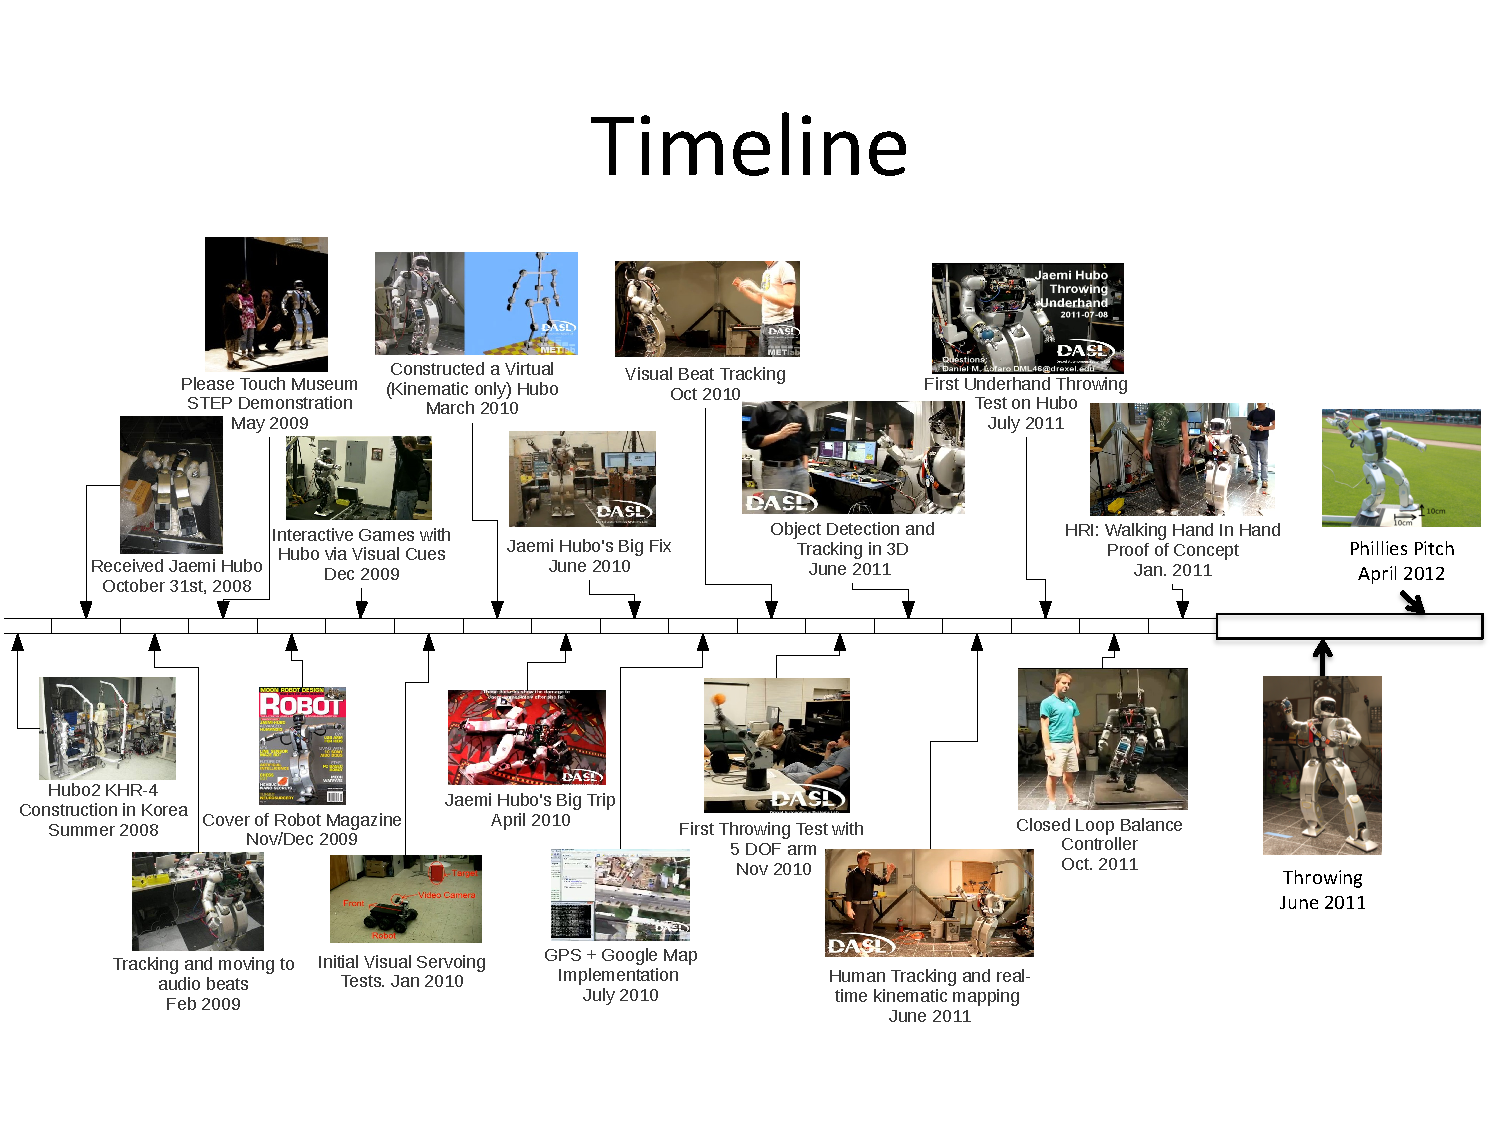
\includegraphics[angle=90, width=0.9\columnwidth]{./pix/Timeline.pdf}
  \caption{Timeline of Daniel M. Lofaro's research from 2008 to 2012}
  \label{fig:timeline}
\end{figure}

\subsection{Human Robot Interaction}
The initial goal was to have a humanoid robot become an interactive musical participant with humans.
This spawned the creation of a visual method of tracking the beat in the absence of auditory cues\cite{5686847}.
This came from a modification of a method of allowing children to play interactive games with humanoid robots\cite{lofaroGamesRobot}.
The resulting method was effective, but to increase the accuracy it was required to combine a pre-existing auditory beat tracker with the visual system.
This calumniated with a multi process system that combine the auditory and visual beat trackers\cite{lofaroIASTED2011,6094987,lofaroEURASIP2011}.
A human comparison was completed and found that this combined method was as accurate at detecting the beat in music as average humans.

\subsubsection{Results from preliminary experiments}
When collaborating with other to create a complex robot control systems integrating controllers is difficult because of the use of:
\begin{itemize}
\item different loop rates causing synchronization issues
\item different programming languages making using the same libraries a challenge
\end{itemize}

It was found that it is best to keep each working systems \textit{independent} allowing them to run at their native rate and on their native platforms\cite{ach}.



\subsection{High Degree of Freedom Kinematic Planning}
The next challenge was to perform kinematic planning for end effector velocity control. 
This resulted in the development of a method that is able to solve inverse kinematics (IK) for high degree of freedom (DOF) systems where there is no closed-form solution as well as create collision free trajectories for high DOF robots\cite{6385987}.
This is described in detail in Section~\ref{sec:srm} and \ref{sec:baseball}.
This culminated in the verification and validation of the system by an experiment where Hubo full-size humanoid robot throw the first pitch at a Major League Baseball (MLB) game\cite{lofaroHumanoids2012,6462956}.

\subsubsection{Results from preliminary experiments}
As best practice when controllers and planners are implemented it is important that low-level controllers such as balance and obstacle avoidance run at all times\cite{lofaroRAM2013}. 
Non-priority controllers such as throwing trajectory planning can run in the background in a separate process.
Keeping the processes separate allowed the system to be more resistant to lag and crashes of one or more of the controllers.
This brought validation to the overarching plan for the unified algorithmic framework for complex systems and humanoid robots.




\subsection{Lessons Learned}

At this point creating these experiment it was required to \textit{hacked} together pre-existing systems that allowed the robot to do the task.
This is the point where it was realized that a \textit{unified algorithmic framework for complex systems and humanoid robots} was required for further development in the field.
Key lessons learned from these experiments were:
\begin{itemize}
\item Must inherently decouple controllers loop rates and phases
\item Must allow for collaborators not have to \textit{inject} their code into existing source.
\item Must work with multiple robots for testing, evaluation, validation, and verification.
\end{itemize}

\noindent This is where Hubo-Ach was born.
The idea was to create a multi process architecture for humanoid control using state of the art high-speed low-latency Inter-Process Communication (IPC) techniques\cite{lofaroRAM2013}.
This is different from traditional IPC techniques because of the lack of head of line (HOL) blocking and focus on low-latency.
Section~\ref{sec:ipc} gives further details and comparisons of different IPCs.


The need for this unified framework was amplified when the Hubo was chosen to be the primary platform for the DRC-Hubo\footnote{DRC-Hubo: http://www.drc-hubo.com/} Track-A team.
Since its initial conception Hubo-Ach has become a fully functional system used in active research by multiple universities including MIT, WPI, Purdue, Ohio State, Swarthmore College, Georgia Tech, and Drexel University\cite{lofaroTePRA2013HuboAch,lofaroTePRA2013Valve}.
This research also acts as a key source of verification and validation of the system.



%%------ About Hubo -------%%
	\section{Primary Platform: Hubo2 Plus}\label{sec:hubo}
			%\subsubsection{Hubo2 Plus}
The Hubo2+ is a $1.3\meter$ (4' 3'') tall, 42 $kg$ (93 $lb$) full-size
humanoid robot.  The Hubo series was designed and constructed by the
Korean Advanced Institute of Science and Technology (KAIST) and
spinoff Rainbow Inc. \cite{hubofirst}.  It has 38 degree of freedom:
six per arm and leg, five per hand, three in the neck, and one in the
waist.  Sensors include three-axis force-torque sensors in the wrists
and ankles, accelerometers in the feet, and an inertial measurement
unit (IMU).  The sensors and embedded motor controllers are connected
via a Controller Area Network to a pair of Intel Atom PC104+ PCs
running a GNU/Linux distribution.



% The reference commands for
% all of the joints are sent from the primary control computer (x86) to
% the individual motor controllers via two Controller Area Network (CAN)
% buses.  This is the same communications bus found in most modern motor
% vehicles.  There are currently eight Hubo's functioning in the United
% States as of December 2012.  Four reside at Drexel University and one
% at Georgia Tech, Purdue, Ohio State and MIT.  Jaemi Hubo is the oldest
% of the Hubos in America and has been at the Drexel Autonomous Systems
% Lab\footnote{Drexel Autonomous Systems Lab:
%   http://dasl.mem.drexel.edu/} (DASL) since 2008 \cite{jaemiHuboSRM}.
% Fig.~\ref{fig:hubo} shows the major dimensions of Hubo.

% \begin{figure}[thpb]
%   \centering
% \includegraphics[width=1.0\columnwidth]{./pix/huboSkel.pdf}
%   \caption{Hubo2 Plus platform: 38 DOF, 130 $cm$ tall full-size humanoid robot weighing 37 $kg$.}
%   \label{fig:hubo}
% \end{figure}

% All joints of the major joints are high gain PID position
% controlled with the exception of the fingers.  The fingers are
% open-loop PWM controlled.
% The sensing capability consists of a three
% axis force-torque (FT) sensor on each leg between the end of the ankle
% and the foot as well as between the arm where it connects to the hand.
% Additionally it has an inertial measurement unit (IMU) at the center
% of mass and accelerometers on each foot.

%%% Local Variables:
%%% mode: latex
%%% TeX-master: "ach"
%%% End:

%%%                                      Sensors Chosen
%%%                                      \begin{itemize}
%%%                                      \item FT
%%%                                      \item IMU
%%%                                      \item Monocular
%%%                                      \item RGB-D
%%%                                      \end{itemize}
	%% Need to add Sensors chosen - ft, imu, monicular, stereo, rgb-d	




%%------ Inspiration -------%%	
	\section{Inspiration: DARPA Robotics Challenge}\label{sec:drc}
    	In July 2012 DARPA released a solicitation for proposals to compeat in the DARPA Robotics Challenge (DRC).
The DRC is a challenge that is in direct response to the Tsuanmi in Psuicima in 2010 (check this).
The challenge is to have a robot be able to use human tools, human vehicles and proform human tasks in an un-structured un modified human enviroment.
We applied for the grant.
In October 2012 we received word that we are a Track-A team for the DRC.
This means that we are competing agains NASA, Raythion, CMU and a team from Japan.
One of the keys to our team is our collaberation.
We are partnered with WPI, Georgia Tech, University of Delleware, Swarthmore, Purdue, Ohio State (check that) and RAINBOW (a company that rose from the Hubo Lab at Korea Advanced Institute of Science and Technology (KAIST)).
Each partner would be responsiable with one event.
We will then combine our efforts into one master controller that is cabiable of doing all the given tasks.
Having a multi-process system that also gives us the ability for our partners to share their controllers without having to intergrate their code.  
Controllers run indipendently.
	
    	%% Add DRC Pix	

%%------ Virtical Leap  -------%%	
    	\section{Controbutions and Vertical Leap}
		The primary contributions and vertical leap to the field is the creation of a \textit{unified algorithmic framework for high degree of freedom complex systems and humanoid robots}.
The resulting framework allows seamless integration of:
\begin{itemize}
\item Controllers running at different loop rates
\item Runs on multiple robots with no modification
\item Runs on simulated robots with no modification 
\item Inherent structure makes it more robust
\item Written in C for controller programing language interdependence (use C bindings in desired language)
\end{itemize}
The unified frame work Hubo-Ach is an Open-Source BSD licensed software allowing for open use.

The contributions of Hubo-Ach have been independently verified by external parties\cite{tepraDoor2013,tepraCut2013}.
Is has been validated by multiple IEEE publications\cite{lofaroTePRA2013HuboAch,lofaroTePRA2013Valve}, in review for a publication in the IEEE Robotics and Automation Society Magazine (RAM)\cite{lofaroRAM2013} and has been the top featured video on the IEEE Spectrum \textit{Video Friday} article on December 14$^{th}$, 2012\cite{videoFriday}.

		%% Works with other stuff


	
%%------ Outline of Document -------%%	
	\section{Document Outline} 
	%% NEED TO WRITE OUTLINE
	
%%------ Into To related Work ------%%
	%% this part of the document should include
		% Hubo-Ach
		% Throwing
		% IK
	%% it might belong just in the "Document Outline" part
			
			
			
			
			
			
%%--------------------
%%-------------------- Below this does not belong in this chapter
%%--------------------
			

		
	\section{Background}\label{sec:background}

This section gives brief background of the methods used for my these.
Section~\ref{sec:back:hubo-ach} describes why inter-process communication (IPC) is used for the Hubo-Ach control system and a brief background of different IPC methods.
Section~\ref{sec:hubo-ach} give this background in greater detail.
Section~\ref{sec:back:ik} and \ref{sec:back:eefvelos} gives the background for the methods used for inverse kinematics and throwing on high DOF robots.
This is the background to the development of the control system that made Hubo throw the first pitch at a Major League Baseball game in 2012 as seen in Section~\ref{sec:hubo-ach} and multiple examples given in Section~\ref{sec:simpleExamples}.
Finally Section~\ref{sec:zmp} gives a brief description of the Zero Moment Point criteria which is used for humanoid walking and shown in the examples in Section~\ref{sec:simpleExamples}.

		
		\subsection{Hubo-Ach: Multi-Process and Interprocess Comunication}\label{sec:back:hubo-ach}
`	    		
This section gives a quick background to why inter-process communication (IPC) is used for the Hubo-Ach control system and a brief background of different IPC methods.
Section~\ref{sec:hubo-ach} give this background in greater detail.

The idea for a Control Architecture for High DOF robots stems from a gap in physical implementation of control algorithms for robot hardware.
The simplest approach to developing robot software is to integrate all functionality in one program.  
This functionality includes the following controllers:
\begin{multicols}{2}
\begin{itemize}
\item Hardware Control
\item Perception
\item Planning
\item Kinematics
\item etc.
\end{itemize}
\end{multicols}

If all of this functionality is in one process then it has the benefit of freedom of inter process communication latency.
However being in one process also means that if one of the controllers lags or faults it cause the entire controller to lag or fault.
This is of great concern if a non-priority controller such as vision processing faults causing a priority controller such as a balance controller, to fail.
This will cause the robot to fall.
How is this fixed?
One solution and my proposed solution is to use multiple processes and IPC methods.
Inter-process communication is a method of exchanging data between multiple processes.
Typical POSIX methods give you the \textbf{oldest} information first and have locks on the memory when processes are writing to it.
An overview of these mechanisms are given in \cite{stevens2005advanced}.

Robots work in the physical world. 
More recent information is more important to it then older.
In most cases it is acceptable to know the most recent data and never read any of the older data.
This would happen if your sensors update at a faster rate then that of the robot.
Typically robot actuators have a bandwidth much much lower then that of a modern computer.
If sensor information is shared using traditional shared memory over POSIX methods the controller would have to read the older information before it reaches the information it is most interested in, the newest data.
This is known effect but new concern for robot controllers called head of line blocking\cite{ach}.

It is desired to make a multi-process controller that can share data between multiple processes with low-latency and no head of line blocking.
There are a few IPCs that offer no head of line blocking and low-latency.  
A description of each IPC type is in Section~\ref{sec:hubo-ach}.
Table~\ref{table:ipc} shows a full comparison of the different IPC types.
%After much research (inserte examples here) it was found that the Ach IPC wuld best fit my needs.

My thesis Hubo-Ach is a multi-process control system that uses IPC methods to communicate between processes.
Section~\ref{sec:hubo-ach} describes Hubo-Ach in detail.



		\subsection{Kinematic Planning}\label{sec:back:ik}
			%% Need more citations
% do parks paper
% do IK
Kinematic planning focuses on creating and testing valid trajectories for series kinematic manipulators.
The focus of this research is on high degree of freedom (DOF), high-gain, position controlled mechanisms.
High-gain position controlled mechanisms are the focus because the experimental platform used for this work is a that type of robot.
This limits the work because it is crucial that the joint-space acceleration profile is correct or the system will over-torque and shutdown.


The works are chosen as it pertains to end-effector velocity control.
Throwing and hitting are examples of end-effector velocity control.  
The goal is to have the end-effector moving at a specific rate in a specific direction.
In most cases it demands whole-body coordination to achieve a desired end-effector velocity.  
Whole-body coordination is different for planted robots and un-planted robots.  


\noindent \textit{Fixed robots} are robots where the base is attached to the ground or the base is significantly more massive then the manipulator.
Planted robots do not have to worry about balance consternates. 

\noindent \textit{Un-fixed robots} are robots that have an manipulator that is not significantly lighter then the base.  
In addition the robot is not physically attached to the ground.
This results in the robot needing to satisfy balance constraints.
In the static case if the robot satisfies the zero moment point (ZMP) criteria it will remain stable~\cite{5686276}.
When the manipulator moves quickly, as in the case of pitching or throwing, such upper-body motions if not coordinated with the lower-body, can cause the humanoid to lose balance.  



%The goal of this work is to show the creation of collision free trajectories for end-effector velocity control, the first step in our overarching goal of creating a system with the ability to throw objects and retain balance.  Towards this, Section~\ref{sec:selfCollision} will discuss our method of detecting self collisions.  Section~\ref{sec:rarea} describes the creation of the robot's sparse reachable map (SRM), a map in $R^3$ of the reachable points. through setting random values to the robot in joint space that takes into account joint limitations and self collisions.  Section~\ref{sec:trajGen} shows the creation of a throwing trajectory in $R^3$ and placing it withing the robot's reachable area using the SRM.  Section~\ref{sec:ik} explains the inverse kinematics used to convert the throwing trajectory in $R^3$ to joint space for this high degree of freedom humanoid robot.  Section~\ref{sec:trap} describes the creation of the approach from the initial pose to the starting pose of the throwing trajectory using a variant of trapezoidal motion control to keep within the actuators' physical limitations.  Section~\ref{sec:exp} features experiments to demonstrate the successful execution of this paper's goal.  Section~\ref{sec:conc} concludes the paper and comments on future work.

		\subsection{End-Effector Velocity Control}\label{sec:back:eefvelos}
			End-effector velocity control (EEVC) is the act of moving your manipulator at a given speed through space at a given velocity.
EEVC is being looked at as the mass of the end-effector does not change.
Thus by controlling the velocity we also control the inertia.
In addition I will be exploring EEVC as it pertains to manipulating objects.
Through my research I have found that end-effector velocity control can be broken up into four major categories:
\textit{Time and location sensitive}, \textit{location sensitive}, \textit{time sensitive}, and \textit{time and location insensitive}.\\


\noindent \textbf{Time and Location Sensitive}: 
If the velocity controler is time and location sensitive it means that your end effector needs to have a given velocity at a specific time in a specific location or the task fales.
Hitting a baseball with a bat is an example of \textit{time and location sensitive}  EEVC.
If the bat has the correct velocity but not at the correct time it will not hit the ball or the ball will not go in the desired place.  
The same goes for if it does not have the correct location but does have the correct velocity.
It is important to note that the manipulator only has instantaneous control over the object at the instant of contact.
Other examples include playing the piano, hitting a tennis ball with a racquet, a moving soccer ball with a foot or any other task that requires to \textit{hit} a \textit{moving} object.\\


\noindent \textbf{Location Sensitive}:
If the velocity controler is location sensitive it means that it only matters that the velocity occurs at a given location.
The time it takes to reach that velocity will not effect the results.
Hitting a nail with a hammer is a prime example of location sensitive EEVC.  
The nail is not moving but it does need to be hit in a given location with a given velocity.
The vector of the velocity is determined by the required angle the nail needs to be hit at.
In this example the nail is not time dependent and can be hit any time.
Hitting it a $t=N$ or $t=N+1$ will not effect the results.
It is important to note that the manipulator only has instantaneous control over the object at the instant of contact.
Other examples of location sensitive end-effector velocity control are hitting a golf ball with a club, hitting a pool ball with the cue, and other activities that require a given location and direction of manipulation but are not time dependent.\\


\noindent \textbf{Time Sensitive}: 
If the location were the end-effector achieves a given velocity is not required to complete the task but the time when it happens is required it is considered \textit{time sensitive} EEVC. 
This means that the end-effector can move in any region it desired as long as the end effector achieves a given velocity at a given time.
The end-effecter's velocity can be dependent on the location achieved but the location is an independent variable and the velocity is the dependent variable.
It is important to note that the manipulator control over the object during the entirety of the motion.
This typically means that the manipulator is holding the object until the release stage.
An example of this is throwing a baseball to first base to get someone out.
Throwing the ball side arm, over arm, or even underarm does not matter as long at it is released at the correct time with the correct velocity to get it ball to the first-baseman to get the runner out.
Other example of time sensitive EEVC are any other instance where an object is thrown within a given time. \\




\noindent \textbf{Time and Location Insensitive}:
If the location and the time of when the end-effector achieves a given velocity does not matter it is considered time and location insensitive.  
The end-effecter's velocity can be dependent on the location achieved but the location is an independent variable and the velocity is the dependent variable.
In this case the manipulator has control over the object until the release stage.
Examples of this would be pitching a baseball, bowling, throwing a grenade or horseshoes etc.
Throwing is an example of when the end-effector's velocity holds a higher priority over the position.  


Mechanisms with only a single degree of freedom are restricted to throwing in a plane.   2-DOF mechanisms are able to throw in $R^3$ space with the correct kinematic structure.
Such a mechanism can choose its release point or its end-effector velocity but not both.
Mechanisms containing 3 or more DOF with the correct kinematic structure are able to throw in $R^3$ and choose both the release point and the end-effector velocity simultaneously. 

In recent work Mori et al. \cite{5152525} has show his ability to control the translational velocity, angular velocity and direction in a 2-dimension plane independently with a single DOF mechanism.
The only input is torque to the manipulator.
The concept consists is to map the input torque that will change only one of the kinimatic variables and not the other two.
This map is done over a given space and thus you can independently chose your translational and angular velocity as well as direction as long as it is in the valid search space.
%The manipulator and a search space example can be seen in Fig.~\ref{fig:mori}. 

%\begin{figure}[thpb]
%  \centering
%\includegraphics[width=0.4\columnwidth]{./background/pix/mori2.png}\includegraphics[width=0.4\columnwidth]{./background/pix/mori1.png}
%  \caption{Map of the input torque that will change only one of the kinimatic variables and not the other two.
%This map is done over a given space and thus you can independently chose your translational and angular velocity as well as direction as long as it is in the valid search space.}
%  \label{fig:mori}
%\end{figure}


Senoo et al.\cite{4651142} used a torque controlled 3-DOF arm to create a high speed throwing trajectory.
This arm falls into the \textit{time and location insensitive} category of throwing.
Senoo used a kinematic chain approach based on how humans throw.  
Doing this Senoo was able to achieved an end-effector velocity of 6.0 $m/s$ and can throw in $R^3$ space.
This is done via the use of a planted robot arm made by Barret Technology Inc consisting of 3-DOF with a $360^o$ rotation base yaw actuator.%, see Fig.~\ref{fig:senoo}. 
 

%\begin{figure}[thpb]
%  \centering
%\includegraphics[width=0.6\columnwidth]{./background/pix/senoo2.png}\includegraphics[width=0.4\columnwidth]{./background/pix/senoo1.png}
%  \caption{3-DOF arm achieving an end-effector velocity of 6.0 $m/s$ and can throw in $R^3$ space.
%This is done via the use of a planted robot arm made by Barret Technology Inc with a $360^o$ rotation base yaw actuator}
%  \label{fig:senoo}
%\end{figure}
 

Low degree of freedom throwing machines/robots are common.  
Typical throwing robots have between one and three degrees of freedom (DOF)~\cite{509405, Lynch97dynamicnonprehensile, 5152525, 509335, springerlink:10.1007/s10015-006-0401-0,throw5347013,throw6386000,throw5152438,throw5423199,throw6224565,throw6347845,throw6071965}.
All of these mechanisms are limited to throwing in a plane.   



These low degree of freedom throwing robots are either physically attached/planted to the mechanical ground or have a base that is significantly more massive then the arm.  



Haddadin et al.\cite{6094757} used their 7-DOF arm and a 6-DOF force torque sensor with standard feedback methods to dribble a basket ball.  
In addition Zhikun et al.~\cite{6094892} used reinforcement learning to teach their 7-DOF planted robot arm to play ping-pong.  
Likewise Schaal et al.~\cite{schaal01/BIRG} taught their high degree of freedom (30-DOF) humanoid to hit a tennis ball using an on-line special statistical learning methods.
Visual feedback was used in the basketball throwing robot by Hu et al.~\cite{5649335} achieving accuracy of 99\%.  
All of the latter robots were fixed to the ground to guarantee stability.

Kim et al. \cite{5686315,JooH2011438} takes the research to the next level with finding optimal overhand and sidearm throwing motions for a high degree of freedom humanoid computer model.  The model consists of 55-DOF and is not fixed to mechanical ground or a massive base.  Motor torques are then calculated to create both sidearm and overhand throws that continuously satisfies the zero-moment-point stability criteria~\cite{4309277}.  

The above works require forms of inverse kinematics.
Most of the works use manipulators less then 6 or 7 DOF.
This is because for those that have less then 6 DOF (7 DOF in some cases) closed form solutions can be solved for\cite{ik5163900,5649842,ik97878,ik326569,ik1087114}.

For higher DOF IK solving methods such as Constrained Bi-directional Rapidly-Exploring Random Tree (CBiRRT) \cite{Berenson_2009_6309}, neural nets\cite{ik23979,ik845162,ik131985,ik832704,ik1662342,ik932681} or learning methods\cite{ik4543497} could be used.
These methods do not guarantee any convergence and/or stability of the solution.

For high DOF IK to guarantee convergence if there is a solution it is possible to use the inverse Jacobian transpose IK solving method\cite{ik99999,ik844073,ik973374,ik4655620}.
Using this iterative method requires that there is only a small change from the end effector's current position and the goal position.  
If the latter is the case, the solver will converge on a solution if one exists.
It is important to note that the initial configuration must be known to obtain a solution.

The end-effector velocity control technique described in Section~\ref{sec:sec:srm} uses the principles of the inverse Jacobian transpose IK method along with forward kinematics and Lofaro et. al.\cite{6385987} Sparse Reachable Map (SRM) to create a high DOF work space end-effector velocity controller.







%			\input{background/FaultDetection.tex}
		\subsection{Balancing: Zero-Moment-Point (ZMP)}\label{sec:zmp}
			\section{Balancing: Zero-Moment-Point (ZMP)}\label{sec:zmp}
The past years of research in humanoids robotics has resulted in a stability criteria that must be followed for bipedal robots to stay stable.
This is known as the Zero Moment Point criteria commonly referred to as ZMP \cite{zmp35}.
ZMP is ubiquitous in the humanoid robotics community.
The ZMP criteria states that a system is statically stable (balanced) if there is no moment acting on the connection between the end effectors touching the ground and the ground.
This means that if the center of mass is over the support polygon there will be no moment.
The support polygon is defined by the are formed by connecting the out most portions of the end effectors (typically feet) that are touching the ground and/or walls, rails etc. 
If the zero moment point, the location of the center of mass (COM) projected in the direction of gravity, is located within this support polygon then the system is considered statically stable.
Fig.~\ref{fig:zmp} gives an example of the zero moment point on a bipedal robot in a single support phase and a double support phase.


\begin{figure}[thpb]
  \centering
\includegraphics[width=0.5\columnwidth]{./background/pix/zmp.png}
  \caption{Example of the zero moment point on a bipedal robot in a single support phase (bottom) and a double support phase (top).  
If the zero moment point, the location of the center of mass (COM) projected in the direction of gravity, is located within this support polygon then the system is considered statically stable.}
  \label{fig:zmp}
\end{figure}

\noindent \textbf{Single Support Phase}:
The single support phase of a bipedal robot is when a single foot is touching the ground.
This creates a smaller support polygon.

\noindent \textbf{Double Support Phase}:
The double support phase of a bipedal robot is when two feed of a bipedal robot are on the ground.
This creates a larger support polygon.  
In addition there is a stable path that the ZMP can move from above one foot to the other.
This allows the robot to guarantee stability while walking (static walking).


		%% add other system comparisions?
	

